\documentclass[10pt]{article}

%\usepackage[latin1]{inputenc}
%\usepackage[english]{babel}
\usepackage{graphicx}
\usepackage{color}
\usepackage{amsmath}
\usepackage{amssymb}
\usepackage{hyperref}
\usepackage{pbox}

\setlength{\parindent}{0cm}

\oddsidemargin -0in%5mm
\evensidemargin -0in%5mm
\topmargin -0.7in%-0.8in%-10mm
%\textheight 9.5in%9.5in%230mm
\textheight 9.3in
\textwidth 6.4in%150mm

%\pagestyle{empty} 

\begin{document}

\clubpenalty1000000
\widowpenalty1000000

%\hyphenpenalty=10000
%\sloppy

\hyphenation{}


\newcommand{\lkon}{\begin{color}{blue}}
\newcommand{\lkoff}{\end{color}}
\newcommand{\here}{\lkon HERE \lkoff}

\newcommand{\spc}{\vspace{0.5cm}}
\newcommand{\spcp}{\vspace{0.2cm}}

\newcommand{\tsize}{\large}


\newcommand{\ug}{$^*$}
\newcommand{\ugshift}{\hspace*{-0.835cm}}
\newcommand{\gr}{$^\dagger$}
\newcommand{\grshift}{\hspace*{-0.835cm}}
\newcommand{\shift}{\hspace{-0.675cm}}

\vspace*{-0.3in}
\makebox[1.072\linewidth][c]
{
%\begin{figure}
  %\vspace{-0.3in}
%\hspace{-1cm}
%\begin{minipage}{0.3\columnwidth}
%\flushleft
%\includegraphics[height=0.8in,trim = 7.295cm 3.53cm 1.24cm 1.18cm, clip]%0.9in]
%{CSUF_logo}
%\end{minipage}
%\hfill
\begin{minipage}{0.5\columnwidth}
  %\flushright {\LARGE Alain Plattner}\\
  \centering {\LARGE Alain Plattner}\\
  \lkon\url{amplattner@ua.edu}\lkoff\\
  \lkon\url{http://alainplattner.net}\lkoff\\
\end{minipage}
%\hfill
%\hspace*{1cm}
%\begin{minipage}{0.3\columnwidth}
%  \flushright
%  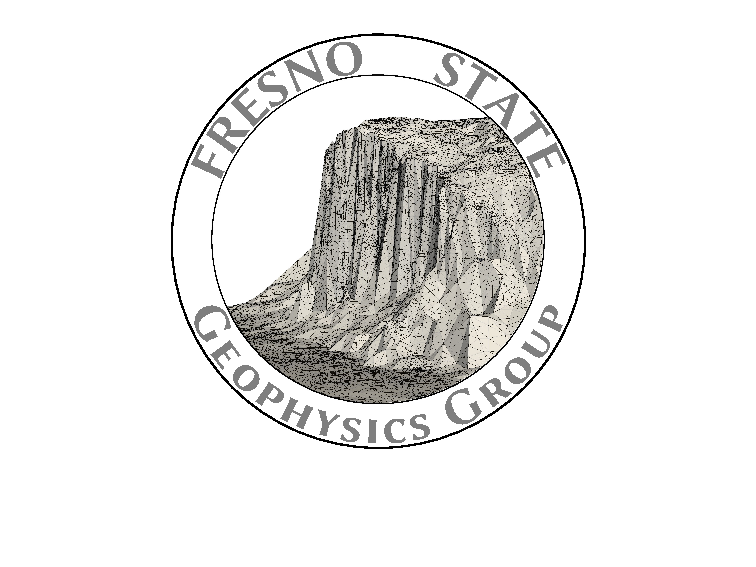
\includegraphics[height=0.8in,trim = 2.85cm 2cm 2.85cm 0.5cm,clip]{FSGG_logo}
%\end{minipage}
%\end{figure}
}



\vspace*{1cm}
\textbf{\tsize CV date:} {\tsize \today}

\spcp
For the most recent version of my CV, click \href{https://github.com/AlainPlattner/CV/blob/master/Plattner_CV.pdf}{\lkon\underline{here}\lkoff}

\spc
\textbf{\tsize Expertise:}

\spcp Planetary magnetic fields. Regional inversion of satellite
magnetic data. Regional spherical-harmonic spectral analysis.
Electrical resistivity tomography. Ground penetrating radar. Near-surface geophysics.

\spc
\textbf{\tsize Address:}

\spcp
Department of Geological Sciences\\
University of Alabama\\
Box 870338\\
Tuscaloosa, AL 35487, USA

%% \spcp
%% Department of Earth and Environmental Sciences\\
%% California State University, Fresno\\
%% 2576 E. San Ramon Ave., Mail Stop ST-24\\
%% Fresno, CA 93740


\spc
\textbf{\tsize Positions:}

\spcp
2018--present:
Assistant Professor at the Department of Geological Sciences, \\University of Alabama, Tuscaloosa AL, USA

\spcp
2014--2018:
Assistant Professor at the Department of Earth and Environmental Sciences, \\California State University Fresno, Fresno CA, USA

\spcp
2011--2014:
Postdoctoral Researcher at the Department of Geosciences, \\Princeton University, Princeton NJ, USA
%Research topic: Development of vectorial Slepian functions and their application to the estimation of crustal magnetization from satellite data.


\spc
\textbf{\tsize Degrees:}

\spcp
\par{2011:} PhD (Dr. Sc. ETH Zurich) in Geophysics at the Institute of Geophysics,
ETH Zurich, Switzerland.
Thesis title: \emph{ Adaptive wavelet methods for geoelectric modelling and inversion}.
Adviser: Prof. Hansruedi Maurer.
doi: 10.3929/ethz-a-006481159

\spcp
\par{2006:} Master of Science in Mathematics at the Institute of Mathematics,
 University of Basel, Switzerland.
 Majors: Algebraic geometry, numerical mathematics

 \spcp
\par{ 2004:} Bachelor of Science in Mathematics at the Institute of Mathematics, 
University of Basel, Switzerland.

\spc
\textbf{\tsize Awards:}

\spcp
NASA Early Career Award (2020)


\spc
\textbf{\tsize Publications:}

\spcp
%$^*$: Undergraduate student first author
\ug: Undergraduate student first author\\
\gr: Graduate student first author


\spcp
\emph{Research articles/book chapters:}

\spcp 
\hspace*{-0.26cm} \gr R.\ Kalski, \textbf{A.\ M.\ Plattner} , C.\ L.\ Johnson, and K.\ T.\ Crane. Crustal magnetization source depths north of the Caloris Basin, Mercury. \emph{Geophys.~Res.~Lett.}, in review

\spcp
D.\ M.\ Peterson, C.\ N.\ Jones, \textbf{A.\ M.\ Plattner}, A.\ J.\ Shogren, S.\ Godsey. Using hydrogeomorphic features to quantify structural and functional hydrologic connectivity in a coastal plain headwater stream. \emph{Water Resour.\ Res.}, in revision

\spcp C.\ Wu, C.\ Lu, Y.\ Chen, \textbf{A.\ Plattner}, B.\ Liu, L.\ Shu, Y.\ Zhang. Satellite and Hydrologic Approaches to Unraveling Groundwater Complexity in a Coastal Plain in China. \emph{J.\ Hydrol.}, in review

\spcp
\shift[20] N.\ McGregor, F.\ Nimmo, C.\ Gillmann, G.\ Golabek, \textbf{A.\ Plattner} and J.\ Conrad. Probing the viscosity of Venus' mantle from dynamic topography at Baltis Vallis. \emph{J.~Geophys.~Res.-Planet}, accepted

\spcp
\shift[19]
T.\ McDonald, \textbf{A.\ M.\ Plattner}, C.\ Warren, M.\ Robinson, G.\ Tian. 3D Visualisation of New Hybrid Rotational Ground Penetrating Radar For Subsurface Inspection of Transport Infrastructure. \emph{IEEE T.\ Geosci.\ Remote}, 63  \href{https://doi.org/10.1109/TGRS.2025.3530758}{doi:~10.1109/TGRS.2025.3530758}.

\spcp
\shift[18] \textbf{A.~M.~Plattner}, E.\ Mazarico, C.\ Gerhards (2024). Variable altitude cognizant Slepian functions. \emph{Int.~J.~Geomath.}, 15(16), \href{https://doi.org/10.1007/s13137-024-00257-w}{doi:~10.1007/s13137-024-00257-w}

\spcp
\shift[17] \textbf{A.~M.~Plattner} and C.\ L.~Johnson (2024). Local spherical harmonic power spectra from local magnetic or gravity data. \emph{Geophys.~J.~Int.}, 236(3):1668--1679,  \href{https://doi.org/10.1093/gji/ggad487}{doi:~10.1093/gji/ggad487} 

\spcp
\shift[16] \textbf{A.~M.~Plattner}, C.\ L.~Johnson, M.J. Styczinski, S.D. Vance, A.C. Mills (2023), On Ganymede's Magnetic Quadrupolar Strength. \emph{Planet.\ Sci.\ J.}, 4:134, \href{https://doi.org/10.3847/PSJ/acde7f}{doi:~10.3847/PSJ/acde7f} 

%% \spcp
%% L.~Ojha, Y.~Quesnel, \textbf{A.~M.~Plattner}, S.~Karunatillake and S.~Tikoo,
%% The role of serpentinization in magnetizing the Noachian crust of Mars.
%% \emph{J.~Geophys.~Res.-Planets}, in review

\spcp
\shift[15] \textbf{A.~M.~Plattner}, S.~Filoromo, E.~H.~Blair (2022), Multi-method geophysical
investigation at Snow's Bend, a Mississippian Platform Mound,
\emph{Archaeol. Prospect.}, \href{https://doi.org/10.1002/arp.1866}{doi:~10.1002/arp.1866}

%\newpage
\spcp
\shift[14] V.~Michel, \textbf{A.~M.~Plattner}, K.~Seibert (2022),
A Unified Approach to Scalar, Vector, and Tensor Slepian Functions on the Sphere and Their Construction by a Commuting Operator
\emph{Anal.~Appl.}, 20(5):947--988, \href{https://doi.org/10.1142/S0219530521500317}{doi:~10.1142/S0219530521500317}

\spcp
\shift[13] \textbf{A.~M.~Plattner} and C.\ L.~Johnson (2021),
Mercury's Northern Rise Core-Field Magnetic Anomaly
\emph{Geophys.~Res.~Lett.}, 48(17):e2021GL094695 \href{https://doi.org/10.1029/2021GL094695}{doi:~10.1029/2021GL094695}

\spcp
%\hspace{-0.835cm}
\grshift \gr[12] M.~Pacheco, \textbf{A.~M.~Plattner}, G.~M.~Stock, D.~H.~Rood and C.~J.~Pluhar (2020),
Surface Exposure Dating and Geophysical Tomography of the Royal Arches Meadow Rock Avalanche, Yosemite Valley, California
\emph{Front.~Earth.~Sci.}, 8:372, \href{https://www.frontiersin.org/articles/10.3389/feart.2020.00372/full}{doi:~10.3389/feart.2020.00372} 

\spcp
\hspace{-0.675cm}[11] \textbf{A.~Plattner} (2020), GPRPy: Open-source ground penetrating radar processing and visualization \\software, \emph{The Leading Edge}, 39(5):332--337, \href{https://doi.org/10.1190/tle39050332.1}{doi:~10.1190/tle39050332.1}

\spcp
\hspace{-0.835cm}$^*$[10] A.~R.~Robbins, \textbf{A.~Plattner} (2018),
Offset-electrode profile acquisition strategy for
electrical resistivity tomography,
\emph{J.~Appl.~Geoph.}, 151:66--72, \href{https://www.sciencedirect.com/science/article/pii/S0926985117308376?via%3Dihub}{doi:~10.1016/j.jappgeo.2018.01.027} 


\spcp
\hspace{-0.5cm}[9] \textbf{A.~Plattner}, F.~J.~Simons (2017),
Internal and external potential field estimation
from regional gradient data at varying satellite altitude,
\emph{Geophys.~J.~Int.}, 211(1):207--238, \href{https://academic.oup.com/gji/article-lookup/doi/10.1093/gji/ggx244}{doi:~10.1093/gji/ggx244} 

\spcp
\hspace{-0.5cm}[8] \textbf{A.~Plattner}, F.~J.~Simons (2015),
High-resolution local magnetic field models for the
Martian South Pole
from Mars Global Surveyor data,
\emph{J.~Geophys.~Res.-Planet}, 120:1543--1566,
\href{http://onlinelibrary.wiley.com/doi/10.1002/2015JE004869/abstract}{doi: 10.1002/2015JE004869}

\spcp
\hspace{-0.5cm}[7] C.~Harig, K.~W.~Lewis, \textbf{A.~Plattner}, and F.~J.~Simons (2015),
A suite of software analyzes data on the sphere,
\emph{Eos Trans.~AGU}, 96(6):18--22,
\href{https://eos.org/project-updates/a-suite-of-software-analyzes-data-on-the-sphere-2}{doi: 10.1029/2015EO025851}

\spcp
\hspace{-0.5cm}[6] \textbf{A.~Plattner} and F.~J.~Simons (2015),
Potential field estimation using scalar and vector Slepian functions at satellite altitude,
\emph{Handbook of Geomathematics, 2nd edition},
\href{https://link.springer.com/referenceworkentry/10.1007\%2F978-3-642-27793-1_64-2}{doi: 10.1007/978-3-642-27793-1\_64-2}

\spcp
\hspace{-0.5cm}[5] F.~J.~Simons and \textbf{A.~Plattner} (2015),
Scalar and vector Slepian functions, spherical signal estimation and spectral analysis,
\emph{Handbook of Geomathematics, 2nd edition},
\href{https://link.springer.com/referenceworkentry/10.1007\%2F978-3-642-27793-1_30-2}{doi: 10.1007/978-3-642-27793-1\_30-2}

\spcp
\hspace{-0.5cm}[4] \textbf{A.~Plattner} and F.~J.~Simons (2014),
Spatiospectral concentration of vector fields on a sphere,
\emph{Appl.~Comput.~Harmon.~Anal.}, 36(1):1--22, 
\href{http://www.sciencedirect.com/science/article/pii/S106352031300002X?via\%3Dihub}{doi: 10.1016/j.acha.2012.12.001}

\spcp
\hspace{-0.5cm}[3] \textbf{A.~Plattner} and F.~J.~Simons (2013), 
A spatiospectral localization approach for analyzing and repres enting vector-valued functions on spherical surfaces,
\emph{Proc. SPIE} 8858, Wavelets and Sparsity XV, 88580N,
\href{http://proceedings.spiedigitallibrary.org/proceeding.aspx?articleid=1745029}{doi: 10.1117/12.2024703}

\spcp
\hspace{-0.5cm}[2] \textbf{A.~Plattner}, H.~R.~Maurer, J.~Vorloeper and M.~Blome (2012),
3-D electrical resistivity tomography using adaptive wavelet parameter grids,
\emph{Geophys.~J.~Int.}, 189(1):317--330,
\href{https://academic.oup.com/gji/article-lookup/doi/10.1111/j.1365-246X.2012.05374.x}{doi: 10.1111/j.1365-246X.2012.05374.x}

\spcp
\hspace{-0.5cm}[1] \textbf{A.~Plattner}, H.~R.~Maurer, J.~Vorloeper and W.~Dahmen (2010),
Three-dimensional geoelectric modelling with optimal work/accuracy rate 
using an adaptive wavelet algorithm,
\emph{Geophys.~J.~Int.}, 182(2):741--752,
\href{https://academic.oup.com/gji/article-lookup/doi/10.1111/j.1365-246X.2010.04677.x}{doi: 10.1111/j.1365-246X.2010.04677.x}

%\spc
\clearpage
\emph{Extended abstracts:}


\vspace{0.2cm}
Note: This section only contains multi-page abstracts that resemble short papers, not the short single paragraph abstracts like for AGU. For a list of short abstracts, see Section ``Abstracts since Fall 2018''.

\spcp
\shift [12] L.\ Ojha, A.\ Mittelholz, S.\ Karunatillake, \textbf{A.\ M.\ Plattner}, S.\ Karimi (2024). Eridania Basin on Mars: A Comprehensive Investigation of the Long-Lived Hydrothermal Hypothesis Through Geochemical, Gravitational, Magnetic Analyses and Crater Relaxation Models. \emph{The Tenth International Conference on Mars}, \href{https://www.hou.usra.edu/meetings/tenthmars2024/pdf/3325.pdf}{Abstract 3325}

\spcp
\shift [11] N.~J.~McGregor, F.~Nimmo, C.~Gillmann, G.~J.~Golabek, \textbf{A.~M.~Plattner}, J.~W.~Conrad (2023), Constraining Venus' Convection Regime From Baltis Vallis Topography, \emph{54th Lunar and Planetary Science Conference 2023},
\href{https://www.hou.usra.edu/meetings/lpsc2023/pdf/1724.pdf}{Abstract 1724}


\spcp
\shift [10] \textbf{A.M. Plattner}, A.~C.~Mills and C.~L.~Johnson (2022), How Dipole-Dominant is Ganymede's Core Magnetic Field?
\emph{53nd Lunar and Planetary Science Conference 2022},
\href{https://www.hou.usra.edu/meetings/lpsc2022/pdf/1111.pdf}{Abstract 1111}

%\clearpage
\spcp
\hspace{-0.5cm}[9] R.~I.~Citron, M.~Manga, D.~Hemingway, \textbf{A.~M.~Plattner} (2021),
Are we visiting the coastlines of Mars? Load-corrected paleo-ocean levels at Jezero, Oxia Planum, and Gale,
\emph{52nd Lunar and Planetary Science Conference 2021},
\href{https://www.hou.usra.edu/meetings/lpsc2021/pdf/1605.pdf}{Abstract 1605}

\spcp
\hspace{-0.77cm} \gr[8] A.~C.~Mills and \textbf{A.~M.~Plattner}
(2020),
Regional Power Spectral Estimation with Application to Galileo Data of Ganymede,
\emph{51st Lunar and Planetary Science Conference 2020},
\href{https://www.hou.usra.edu/meetings/lpsc2020/pdf/2264.pdf}{Abstract 2264}

\spcp
\hspace{-0.5cm}[7] \textbf{A.~Plattner}, C.~L.~Johnson (2019), Large-Scale Non-Axisymmetric Internal Structure of Mercury's Magnetic Field,
\emph{50th Lunar and Planetary Science Conference 2019},
\href{https://www.hou.usra.edu/meetings/lpsc2019/pdf/1645.pdf}{Abstract 1645}


\spcp
%\clearpage
\hspace{-0.5cm}[6] \textbf{A.~Plattner}, C.~L.~Johnson (2018),
Regional Modeling and Power Spectra of Mercury's Crustal Magnetic Field,
\emph{Mercury 2018},
\href{https://www.hou.usra.edu/meetings/mercury2018/pdf/6023.pdf}{Abstract 6023}

\spcp
\hspace{-0.5cm}[5] C.~L.~Johnson,
\textbf{A.~M.~Plattner}. R.~J.~Phillips, L.~C.~Philpott, M.~Kinczyk,
L.~Prockter (2018), The Distribution and Origin of Mercury's Lithospheric Magnetization, \emph{Mercury 2018},
\href{https://www.hou.usra.edu/meetings/mercury2018/pdf/6052.pdf}{Abstract
  6052}

\spcp
\hspace{-0.5cm}[4] \textbf{A.~Plattner}, G.~J.~Golabek, F.~J.~Simons (2017),
A spectral view of the Terra Sirenum / Cimmeria crustal magnetic
field,
\emph{48th Lunar and Planetary Science Conference 2017},
\href{http://www.lpi.usra.edu/meetings/lpsc2017/pdf/1627.pdf}{Abstract 1627}

\spcp
\hspace{-0.67cm}$^*$[3] A.~R.~Robbins and \textbf{A.~Plattner}
(2017),
2.75-D ERT: Zigzag electrode acquisition strategy to improve 2-D
Profiles,
\emph{Symposium on the Application of Geophysics to Engineering and
  Environmental Problems 2017}, 183--187,
\href{http://library.seg.org/doi/pdf/10.4133/SAGEEP.30-007}{doi: 10.4133/SAGEEP.30-007}

%\newpage
\spcp
\hspace{-0.5cm}[2] \textbf{A.~Plattner} and F.~J. Simons (2015),
Mars' heterogeneous South Polar magnetic field revealed using altitude vector Slepian functions,
\emph{46th Lunar and Planetary Science Conference 2015},
\href{http://www.hou.usra.edu/meetings/lpsc2015/pdf/1794.pdf}{Abstract 1794}

\spcp
\hspace{-0.5cm}[1] \textbf{A.~Plattner}, F.~J.~Simons, L.~Wei (2012),
Analysis of real vector fields on the sphere using Slepian functions,
\emph{IEEE Statistical Signal Processing Workshop (SSP)},
\href{http://ieeexplore.ieee.org/stamp/stamp.jsp?tp=&arnumber=6319659}{Abstract}

\spc
\emph{Non peer-reviewed publications:}

\spcp
\hspace{-0.5cm}[1] \textbf{A.~Plattner}, M.~Pacheco, (2019), A
community-developed free Ground Penetrating Radar software,
\emph{Near-Surface Views, Newsletter of the Near-Surface Geophysics
  Technical Section of The Society of Exploration Geophysicists},
\href{https://seg.org/Portals/0/SEG/News%20and%20Resources/Near%20Surface/Near%20Surface%20Newsletter/2011-present/2019_Q1.pdf}{Q1
  2019 Newsletter}


\spc
\textbf{\tsize Funding:}

\spcp
Funded: NASA Mars Data Analysis Program [NNH21ZDA001N-MDAP], 2023--2025

\spcp
Funded: NASA Planetary Sciences Early Career Award [80NSSC20K1080], 2020--2024

\spcp Declined: EPSCoR grant proposal 2019

\spcp
Funded: NASA Discovery Data Analysis Program [80NSSC19K1426], 2019--2023

\spcp
Transfer: NSF Geoinformatics [EAR-2022671], 2019--2022 

\spcp
  Funded: NSF Geoinformatics
  %\href{http://www.nsf.gov/awardsearch/showAward?\
  %  AWD_ID=1550732&HistoricalAwards=false}{\lkon[EAR-1550732]\lkoff},
  [EAR-1550732],
  2016--2020

 \spcp 
Funded: NASA Mars Data Analysis Program [NNX14AM29G], 2014--2017

\spcp Funded: Swiss National Science Foundation Fellowship for Prospective Researchers
[PBEZP2-134427], 2011--2012

\spcp
Funded: Ulrich Schmucker Memorial Trust grant (2011)


\spc
\textbf{\tsize Conference Oral Presentations:}

\vspace{0.2cm}
Note: This section only contains presentations where my students or I were first authors. For other co-authored oral presentations, please see section ``Co-authored presentations since 8/2018.

\spcp
%$^*$: Undergraduate student first author
\ug: Undergraduate student presenter and/or first author\\
\gr: Graduate student presenter and/or first author\\
\textbf{bold}: Invited/solicited conference talks

\spcp
\hspace{-0.4cm} \gr \hspace{-0.03cm} On the Range of Magnetic Source Depths of the Terra Cimmeria
and Sirenum region on Mars, R.\ Soltanabadi, \textbf{A.~M.~Plattner},
L.\ Ojha, G.\ Golabek,  \emph{AGU Fall Meeting}, Washington, DC, Dec 2024

\spcp
Investigating Planetary Crustal Magnetic Field Anomalies from
Spacecraft Magnetic Field Measurements using Variable Altitude
Cognizant Slepian Functions, \textbf{A.~M.~Plattner}, E.\ Mazarico,
C.\ Gerhards, \emph{AGU Fall Meeting}, Washington, DC, Dec 2024

\spcp
Geophysical investigation of a $\sim4500$ year old Native American shell ring, \textbf{A.~M.~Plattner}, E.~B.~Blair, A.~Semon, R.~Cajigas, T.~Blaber, M.~Sanger, D.~H.~Thomas,  \emph{AGU Fall Meeting}, San Francisco, CA, Dec 2023

\spcp
\textbf{Ground penetrating radar data processing and visualization using the open source software GPRPy, A.~Plattner. \emph{The International Meeting for
Applied Geoscience \& Energy (IMAGE)}, Houston TX, Aug 2023 (invited)}

\spcp
\hspace{-0.4cm} \gr \hspace{-0.03cm} How Dipole-Dominant is Ganymede’s Core Field? \textbf{A.~M.~Plattner}, A.~C.~Mills, C.~L.~Johnson, \emph{53rd Lunar and Planetary Science Conference},
The Woodlands, TX, March 2022


\spcp
Geophysical Investigation of a Native-American Mound using Time-Domain Induced Polarization, \textbf{A.~M.~Plattner}, S.~Filoromo. E.~H.~Blair, \emph{AGU Fall Meeting}, New Orleans, LA, Dec 2021


\spcp
Non-axisymmetric structure in Mercury's core field, \textbf{A.~Plattner}, C.~Johnson, \emph{Annual Meeting of the Mercury Exploration Assessment Group (MExAG)}, Online, Feb, 2021

%\clearpage
\spcp
\hspace{-0.4cm} \gr \hspace{-0.03cm} \textbf{Near-Surface Geophysical Tomography of the Royal Arches Meadow Rock Avalanche in Yosemite Valley, California, M.~Pacheco, {\normalfont A. Plattner}, G.~M.~Stock, D.~H.~Rood, C.~J.~Pluhar, \emph{AGU Fall Meeting}, Online, Dec 2020 (invited)}

\spcp
\hspace{-0.4cm} \gr \hspace{-0.03cm} The Crust and Upper Mantle Structures in Central Anatolia,Turkey, Constrained by Gravity and Seismic Data, Y.~Y\i lmaz, \textbf{A.~M.~Plattner}, R.~Mahatsente, I.~\c Cemen, B.~Zhang, \emph{GSA Connects}, Online, Oct 2020

\spcp
\hspace{-0.4cm} \gr \hspace{-0.03cm} Three-dimensional Geophysical Imaging of the Royal Arches Meadow Rock Avalanche in Yosemite Valley, California, M.~Pacheco, \textbf{A.~Plattner}, G.~Stock, C.~Pluhar, \emph{AGU Fall Meeting}, San Francisco, CA, Dec 2019

\spcp
Mercury's Large-Scale Non-Axisymmetric Internal Field from MESSENGER Data, \textbf{A.~Plattner}, C.~L.~Johnson, \emph{AGU Fall Meeting}, San Francisco, CA, Dec 2019

\spcp
Large-Scale Non-Axisymmetric Internal Structure or Mercury's Magnetic Field,
\textbf{A.~Plattner}, C.~L.~Johnson, \emph{50th Lunar and Planetary Science Conference},
The Woodlands, TX, March 2019

\spcp
A spectral view of the Terra Sirenum / Cimmeria crustal magnetic field, \textbf{A.~Plattner}, F.J.~Simons, G.~Golabek, \emph{48th Lunar and Planetary Science Conference}, The Woodlands, TX, March 2017

%\newpage
\spcp 
\hspace{-0.4cm}\ug \, \textbf{2.75-D ERT: Zigzag electrode acquisition strategy
to improve 2-D profiles,
A.~R.~Robbins, {\normalfont A.~Plattner},
\emph{23rd European Meeting of Environmental and Engineering Geophysics}, Malmo, Sweden, Sep 2017 (best of SAGEEP invited talk)}

\spcp 
\hspace{-0.4cm} $^*$ 2.75-D ERT: Zigzag electrode acquisition strategy
to improve 2-D profiles,
A.~R.~Robbins, \textbf{A.~Plattner},
\emph{SAGEEP}, Denver, CO, Mar 2017

\spcp
The Crustal Magnetic Field of Terra Sirenum and Cimmeria, Mars. A Spectral Perspective,
\textbf{A.~Plattner}, F.~J.~Simons, G.~Golabek, 
\emph{AGU Fall Meeting}, San Francisco, CA, Dec 2016

\spcp
Teaching Near-Surface Geophysics within the Matlab/Octave Community,
\textbf{A.~Plattner}, 
\emph{AGU Fall Meeting}, San Francisco, CA, Dec 2016

\spcp
Localized Bandlimited Inversion of Planetary Magnetic-Field Data,
\textbf{A.~Plattner}, F.~J.~Simons,
\emph{SIAM Conference on Mathematical and Computational Issues in the Geosciences},
Stanford University, Stanford, CA, Jul 2015


\spcp
\textbf{High-resolution crustal magnetic field model of the Martian South Pole using altitude vector\\ Slepian functions,
\emph{A.~Plattner}, F.~J.~Simons,
\emph{Joint Mathematics Meeting}, San Antonio, TX, Jan 2015 (invited)}

\spcp
\textbf{Planetary potential-field inversion from vectorial data: Using Slepian functions for varying satellite altitude,
\emph{A.~Plattner}, F.~J.~Simons,
\emph{Joint Mathematics Meeting}, Baltimore, MD, Jan 2014 (invited)}

\spcp
\textbf{Regional crustal field modeling from regional satellite data with varying altitude using dedicated vector Slepian functions,
\emph{A.~Plattner}, F.~J.~Simons,
\emph{AGU Fall Meeting}, San Francisco, CA, Dec 2013 (invited)}

\spcp
Signal and Spectral Estimation on a Sphere,
F.~J.~Simons, \textbf{A.~Plattner},
\emph{AMMCS 2013}, Waterloo, ON, Canada, August 2013 (invited speaker: F.J.~Simons)

\spcp
Source field estimation from satellite data using vectorial spatiospectrally 
concentrated functions,
\textbf{A.~Plattner}, F.~J.~Simons,
\emph{Geomathematics 2013}, Sankt Martin, Germany, April 2013

\spcp
\textbf{Vectorial Slepian functions and the estimation of the crustal magnetic field,
A.~Plattner, F.~J.~Simons,
\emph{EGU General Assembly}, Vienna, Austria, April 2013 (solicited)}

\spcp
Vector-valued crustal magnetic field estimation using vector Slepian functions,
\textbf{A.~Plattner}, F.~J.~Simons,
\emph{AGU Fall Meeting}, San Francisco, CA, Dec 2012

\spcp
Geophysical survey of the Peristeries plateau in Polis Chrysochous, Cyprus,
\textbf{A.~Plattner}, F.~J.~Simons, J.~S.~Smith, A.~C.~Maloof, J.~Husson,
\emph{American Schools of Oriental Research Annual Meeting}, Chicago, IL, Nov 2012

\spcp
Adaptive wavelet parameterization for 3d electrical resistivity tomography,
\textbf{A.~Plattner}, H.~R.~Maurer, 
\emph{AGU Fall Meeting}, San Francisco, CA, Dec 2011

\spcp
Adaptive wavelet modeling of geophysical data,
\textbf{A.~Plattner}, H.~R.~Maurer, J.~Vorloeper and W.~Dahmen, 
\emph{AGU Fall Meeting}, San Francisco, CA, Dec 2009



%\clearpage

\spc
%\emph{Seminar talks:}
\textbf{\tsize Seminar Talks:}

\spcp
Technische Universität Bergakademie Freiberg (Germany), Jul 2023\\
Society of Explorational Geophysics Webinar for Open-Source Software, Apr 2023\\
University of Western Washington (USA), Geology Department, Mar 2022\\
University of Toronto (Canada), Department of Earth Sciences and Department of Physics, Feb 2022\\
BepiColombo Geodesy and Geophysics Working Group, Nov 2021\\
University of South Florida (USA), School of Geosciences, Feb 2020\\
University of Mississippi (USA), Department of Geology and Geological Engineering, Oct 2019\\
University of Alabama (USA), Department of Physics and Astronomy, Sep 2019\\
University of Cape Town (South Africa), Department of Geology, Sep 2018\\
NASA Goddard Space Flight Center (USA), Jul 2018\\
University of Siegen (Germany), Department of Mathematics, May 2018\\
University of Alabama (USA), Department of Geological Sciences, Feb 2018\\
SERC Carleton College (Webinar), Apr 2017\\
University of the Witwatersrand (South Africa), School of Geosciences, Jul 2016\\
University of British Columbia (CA), Dept.~of Earth, Ocean and Atmospheric Sci., Feb 2016\\
UC Santa Cruz (USA), Earth and Planetary Sciences Department, Oct 2014\\
Princeton University (USA), Department of Geosciences, Sept  2011, Apr 2014\\
CSU Fresno (USA), Department of Earth and Environmental Science, Feb 2014\\
Princeton University (USA), Program in Appl.~and Comp.~Mathematics, Nov 2013\\
Rutgers (USA), Department of Earth and Environmental Sciences, Feb 2012\\
Cornell University (USA), Department of Earth and Atmospheric Sciences, Feb 2012\\
Universite de Lausanne (Switzerland), Institute de Geophysique, Nov 2009, Jan 2012\\
ETH Zurich (Switzerland), Seminar for Applied Mathematics, Dec 2010\\
ETH Zurich (Switzerland), Department of Earth Sciences, Oct 2009



%\clearpage
\spc
\textbf{\tsize Conference Poster Presentations:}

\vspace{0.2cm}
Note: This section only contains presentations where my students or I were first authors. For other co-authored poster presentations, please see section ``Co-authored presentations since 8/2018.


\spcp
\ug: Undergraduate student first author\\
\gr: Graduate student first author\\
\textbf{bold}: Invited/solicited conference posters

\spcp
\hspace*{-0.4cm} \gr \hspace*{-0.05cm} On the Origin of Mercury's Crustal
Magnetic Field North of the Caloris Impact Basin, R.\ Kalski,
\textbf{A.\ Plattner}, C.~L.~Johnson, K.\ T.\ Crane, \emph{AGU Fall
Meeting}, Washington, DC, Dec 2024

\spcp
\hspace*{-0.35cm} \gr \hspace*{0.02cm} Regional crustal magnetic source depth of the Terra Cimmeria and Sirenum Region on Mars, R.~Soltanabadi, \textbf{A.~Plattner}, C.~L.~Johnson, L.~Ohja, G.~Golabek, \emph{AGU Fall Meeting}, San Francisco, CA, Dec 2023 

\spcp
Revisiting Constraints on Ganymede's Dynamo from Spacecraft Magnetic Field Data,
\textbf{A.~Plattner}, A.~C.~Mills, C.~L.~Johnson, M.~J.~Styczinski, S.~D.~Vance,  \emph{AGU Fall Meeting}, Chicago, IL and online, Dec 2022 

\spcp
Local magnetic field power spectrum from local data,
\textbf{A.~Plattner}, C.~L.~Johnson, 
\emph{AGU Fall Meeting}, Online, Dec 2020 

\spcp
\hspace*{-0.35cm} \gr \hspace*{0.05cm} Geophysical Investigation of the Royal Arches Meadow Rock
Avalanche in Yosemite Valley - CA,
M.~Pacheco, \textbf{A. Plattner},
\emph{GSA Cordilleran Meeting}, Portland OR, May 2019

\spcp
\textbf{Ground Penetrating Radar Data Processing and Visualization using
GPRPy,
\emph{A.~Plattner},\\
\emph{AGU Fall Meeting}, Washington DC, Dec 2018}

\spcp
Mercury's Core Field: Beyond the Offset Axial Dipole,
\textbf{A.~Plattner}, C.~L.~Johnson, 
\emph{AGU Fall Meeting}, Washington DC, Dec 2018 

\spcp
\hspace*{-0.4cm} \gr \hspace*{-0.05cm} Near Surface Geophysical Imaging of the Internal
Structure of El Capitan Meadow Rock Avalanche in Yosemite National
Park, California,
C.~Liu, \textbf{A.~Plattner}, G.~Stock,
\emph{AGU Fall Meeting}, Washington DC, Dec 2018


\spcp
Mercury's Crustal Magnetic Field from MESSENGER Data,
 \textbf{A.~Plattner}, C.~L.~Johnson, 
\emph{AGU Fall Meeting}, New Orleans, LA, Dec 2017 

%\clearpage
\spcp
\hspace{-0.4cm} $^*$ A glimpse in the third dimension for electrical
resistivity profiles,
A.~R.~Robbins, \textbf{A.~Plattner},
\emph{AGU Fall Meeting}, New Orleans, LA, Dec 2017 

%\clearpage
\spcp
\hspace{-0.4cm} $^*$ Electrical Resistivity and Ground Penetrating Radar 
Investigation of Presence and Extent of Hardpan Soil Layers,
 S.~J.~Thao, \textbf{A.~Plattner},
\emph{AGU Fall Meeting}, San Francisco, CA, Dec 2015

\spcp
Localized crustal magnetic field inversion from inner- and outer-source altitude vector Slepian functions, \textbf{A.~Plattner},  F.~J.~Simons,
\emph{AGU Fall Meeting}, San Francisco, CA, Dec 2015


\spcp
Mars' Heterogeneous South Polar Magnetic Field Revealed using Altitude Vector Slepian Functions,
\textbf{A.~Plattner},  F.~J.~Simons,
\emph{46th Lunar and Planetary Science Conference}, The Woodlands, TX, March 2015


\spcp
High-resolution Local Crustal Magnetic Field Modeling of the Martian South Pole,
\textbf{A.~Plattner},  F.~J.~Simons,
\emph{AGU Fall Meeting}, San Francisco, CA, Dec 2014

\spcp
Altitude vector Slepian functions and satellite crustal magnetic field data,
\textbf{A.~Plattner},  F.~J.~Simons,
\emph{3rd Swarm Science Meeting}, Copenhagen, Denmark, June 2014

\spcp
Local gravity field modeling from vectorial satellite data using Slepian functions,
\textbf{A.~Plattner},  F.~J.~Simons,
\emph{AGU Fall Meeting}, San Francisco, CA, Dec 2013

\spcp
Analysis of real vector fields on the sphere using Slepian functions,
\textbf{A.~Plattner}, F.~J.~Simons, L.~Wei,
\emph{IEEE Statistical Signal Processing Workshop}, Ann Arbor, MI, Aug 2012

\spcp
Lithospheric magnetic field reconstruction using vector Slepian functions,
\textbf{A.~Plattner}, F.~J.~Simons,
\emph{Symposium on Study of the Earth's Deep Interior}, Leeds, United Kingdom, July 2012

\spcp
Spatiospectral concentration of vector fields on a sphere,
\textbf{A.~Plattner}, F.~J.~Simons,
\emph{Challenges in Geometry, Analysis, and Computation: High-Dimensional Synthesis}, 
New Haven, CT, June 2012

\spcp
Vector spherical Slepian functions -- spatiospectral concentration of vector fields on the sphere,
\textbf{A.~Plattner}, F.~J.~Simons, L.~Wei,
\emph{AGU Fall Meeting}, San Francisco, CA, Dec 2011

%\clearpage

\spc
\textbf{\tsize Co-authored presentations since 8/2018}


\spcp D.\ Peterson, N.\ Jones, \textbf{A.\ M.\ Plattner}, S.\ Godsey,
A.\ Shogren, Using hydrogeomorphic features to quantify structural and
functionalhydrologic connectivity in a Coastal Plain headwater stream,
AGU Fall Meeting, Washington, DC, Dec 2024. \emph{Oral}

\spcp D.\ Peterson, N.\ Jones, \textbf{A.\ M.\ Plattner}, S.\ Godsey, A.\ Shogren, Using hydrogeomorphic features to quantify structural and functionalhydrologic connectivity in a Coastal Plain headwater stream, Alabama Water Resources Conference, Orange Beach, AL, Sep 2024. \emph{Oral}

\spcp
L.\ Ojha, A.\ Mittelholz, S.\ Karunatillake, \textbf{A.\ M.\ Plattner}, S.\ Karimi, Eridania Basin on Mars: A Comprehensive Investigation of the Long-Lived Hydrothermal Hypothesis Through Geochemical, Gravitational, Magnetic Analyses and Crater Relaxation Models. The Tenth International Conference on Mars, Pasadena, CA, July 2024. \emph{Poster}

\spcp A.\ Semon, R.\ Cajigas, E.\ Blair, M.\ Sanger, \textbf{A.\ M.\ Plattner}, Recent Investigations at the Musgrove Shell Ring (9LI2169) on St. Catherines Island, Georgia, \emph{Society for American Archaeology}, New Orleans, LA, Apr 2024. \emph{Poster}

\spcp N.~J.~McGregor, F.~Nimmo, C.~Gillmann, G.~J.~Golabek, \textbf{A.~M.~Plattner}, J.~W.~Conrad, Dynamic Topography of Baltis Vallis Reveals Low Viscosity of the Venusian Mantle, \emph{AGU Fall Meeting}, San Francisco, CA, Dec 2023. \emph{Poster}

\spcp
A.~Semon, R.~Cajigas, E.~Blair, M.~Sanger, \textbf{A.~M.~Plattner}, C.~O'Shaughnessy, D.~H.~Thomas, Geophysics and excavations at the Musgrove Creek Shell Ring on St. Catherines Island, GA, \emph{Annual Meeting of the Southeastern Archaeological Conference}, Chattanooga, TN, Oct 2023. \emph{Oral}

\spcp C.~Gillmann, N.~McGregor, F.~Nimmo, G.~Golabek, \textbf{A.~M.~Plattner}, J.~Conrad, Constraining Venus' convection regime from Baltis Vallis topography, \emph{55th Annual Meeting of the DPS}, San Antonio, TX, Oct 2023. \emph{Oral}

\spcp N.~J.~McGregor, F.~Nimmo, C.~Gillmann, G.~J.~Golabek, \textbf{A.~M.~Plattner}, J.~W.~Conrad, Constraining Venus' convection regime from Baltis Vallis topography, \emph{EGU General Assembly}, Vienna, Austria, Apr 2023. \emph{Poster}

\spcp N.~J.~McGregor, F.~Nimmo, C.~Gillmann, G.~J.~Golabek, \textbf{A.~M.~Plattner}, J.~W.~Conrad, Constraining Venus' convection regime from Baltis Vallis topography, \emph{54th Lunar and Planetary Science Conference}, The Woodlands, TX, Mar 2023. \emph{Poster}

\spcp H.F.~Rogers, C.~Beggan, K.~Whaler, and \textbf{A.~Plattner}
(2022), Investigating regional heterogeneity at the core-mantle
boundary and its impact on outer core flow by applying spherical
Slepian functions \emph{SEDI Meeting}, Z\"urich, Switzerland, Jul 2022. \emph{Poster}

\spcp D.~Pederson, N.~Jones, A.~Shgoren, \textbf{A.~Plattner},
S.~Godsey, C.~Atkinson, J.~Bernstead (2022). Detangling Tanglewood:
Three-dimensional Hydrologic Connectivity in a Coastal Plain Headwater
Stream. \emph{Joint Aquatic Science Meeting}, Grand Rapids, MI, May
2022. \emph{Poster}

\spcp D.~Peterson, C.~N.~Jones, \textbf{A.M.~Plattner}, A.~Shogren,
S.~Godsey, C.~Atkinson, J.~Benstead (2022), Detangling Tanglewood:
Characterizing vertical, horizontal, and longitudinal hydrologic
connectivity in a Coastal Plain headwater stream. \emph{Mississippi
Water Resources Conference}, Startkville, MS, Apr 2022.  \emph{Oral}

\spcp S.~Filoromo, \textbf{A.~Plattner} and E. Blair (2022), Building
Community in Moundville's Chiefdom: New Insights from Geophysical
Investigations of the Late Mississippian Platform Mound at Snow's Bend
(1Tu2/3). \emph{Society for American Archaeology Annual Meeting}, Chicago,
IL, Mar 2022. \emph{Oral}

\spcp D.~Peterson, C.~N.~Jones, \textbf{A.M.~Plattner}, A.~Shogren,
S.~Godsey, C.~Atkinson, J.~Benstead (2021), Drivers of vertical,
horizontal, and longitudinal hydrologic connectivity in a
non-perennial Coastal Plain stream. \emph{AGU Fall Meeting}, New
Orleans, LA, Dec 2021. \emph{Poster}

\spcp R.~Cajigas, \textbf{A.~Plattner}, E.~H.~Blair (2021),
Geoarchaeological investigations at Mound Z, Moundville, Alabama
(1TU500). \emph{Geological Society of America}, Portland, OR, Oct
2021. \emph{Poster}

\spcp R.~I.~Citron, M.~Manga, D.~Hemingway and \textbf{A.~M.~Plattner}
(2021), Are we visiting the coastlines of Mars? Load-corrected
paleo-ocean levels at Jezero, Oxia Planum, and Gale, \emph{52nd Lunar
and Planetary Science Conference 2021}, Online, March 2021.
\emph{Oral}

\spcp
Localized High-Latitude Inversion of GRACE Level-1 Data Using Slepian Functions,
C.~Harig, Y.~Zhang, C.K. Shum, \textbf{A.~Plattner}
\emph{AGU Fall Meeting}, San Francisco, CA, Dec 2019. \emph{Poster}

\spcp
Regionalized properties of the lowermost mantle from spherical Slepian analysis,
T.~M.~Olugboji, P.~Moulik, \textbf{A.~Plattner}, V.~Lekic
\emph{AGU Fall Meeting}, San Francisco, CA, Dec 2019. \emph{Oral}

\spcp Regionalized Properties of the Lowermost Mantle From Spherical
Slepian Analysis, T.~M.~Olugboji, P.~Moulik, \textbf{A.~Plattner},
V.~Lekic \emph{SSA Annual Meeting}, Seattle, WA, Apr
2019. \emph{Poster}

\spcp 3D numerical models of thermal convection inside Triton’s icy
shell, G.~Golabek, F.~Nimmo, T.~Gerya, P.~Schenk, \textbf{A.~Plattner}
\emph{EGU Annual Meeting}, Vienna (AT), Apr 2019. \emph{Poster}

\spcp 3D numerical models of thermal convection inside Triton's icy
shell G.~Golabek, F.~Nimmo, T.~Gerya, P.~Schenk, \textbf{A.~Plattner}
\emph{AGU Fall Meeting}, Washington DC, Dec 2018. \emph{Poster}





\spc
\textbf{\tsize Teaching:}

\spcp
\textbf{2018 -- today: Department of Geological Sciences,
University of Alabama}

``Computers in Earth Science''

``Introduction Geophysics''

``Hazardous Earth''

``The Dynamic Earth''

%\clearpage
\spcp
\textbf{2014 -- 2018:  Department of Earth and Environmental Science, CSU Fresno}

``Applied Geophysics''

``Natural Disasters and Earth Resources''

``Geoscientific Computing''

``Geophysics Seminar''

``Environmental Earth and Life Science''


\spcp
\textbf{2011--2013:  Department of Geosciences, Princeton University}

Instructor for ``Earth's environments and ancient civilizations''

\spcp
\textbf{2006--2011: Department of Earth Sciences, ETH Zurich}

Teaching assistant for ``Numerical modeling in applied geophysics''
     
Teaching assistant for field courses (electromagnetic prospecting)

\spcp
\textbf{2004--2006: Department of Mathematics, University of Basel}

Teaching assistant for ``Mathematics for natural scientists''

Teaching assistant for ``Linear algebra''


\spc
%\clearpage
\textbf{\tsize Advising:}

\spcp
\emph{PhD Students:}\\
Rezvan Soltanabadi (2022--present) 

\spcp
\emph{MS Students:}\\
Ramon Richardson (2020--2023); 
Alyssa Mills (2019--2023);
Yagmur Yilmaz (2019--2021);
Michaela May (2020--2021);
Marcus Pacheco (2017--2019);
Christine Liu (2016--2018) 

\spcp
\emph{PhD Committee Member Internal:}\\
Olaoluwa Oluwaniyi (2023--present);
Yitao Pu (2023--present);
Taylor Woods (2023);
Hesam Saeidi (2019--present);
Ioannis Kouvatsis (2019--present);
Jordan Faltys (2018--present);
Ashish Kumar (2019--2021);
Virginia Andrews (2018--2020);
Hao Wu (2019)

\spcp
\emph{MS Committee Member Internal:}\\
Nathan Patty (2024--present);
Kayode Agboola (2021--2023);
Steven Filoromo (2020--2022) 

\spcp
\emph{External PhD examiner:}\\
Kathrin Seibert (2018, University of Siegen, Germany);
Timothy Wiese (2012, University of Adelaide, Australia)

\spcp
\emph{External MS examiner:}\\
Tom New (2022, University of Cape Town, South Africa)


\spc
%\clearpage
\textbf{\tsize Service:}

\spcp
Editor for International Journal on Geomathematics (GEM), since 2019

\spcp
Chaired four NASA panels and served on four
additional panels as panelist (total: 8 panels since 2020)

\spcp
Reviewed numerous papers since 2010 for the following journals:\\
\emph{Earth and Space Science},
\emph{Earth-Sci.~Rev.},
\emph{Geophys.~J.~Int.},
\emph{Geophys.~Prospect.},
\emph{Geophys.~Res.~Lett.},
\emph{Geophysics},
\emph{IEEE T.~Signal Proces.},
\emph{Icarus},
\emph{Intern.~J.~Geomath.},
\emph{Int.~J.~Speleol.},
\emph{J.~Appl.~Geophys.},
\emph{J.~Geodesy},
\emph{J.~Geophys.~Res.},
\emph{Mech.~Res.~Commun.},
\emph{Nat.~Commun.},
\emph{Pure~Appl.~Geophys.}

\spcp
Co-organizer of session ``Planetary Magnetism and Protoplanetary Disk Magnetism'' at AGU Fall Meeting 2022 and 2023

\spcp
Principal organizer of session ``Planetary Magnetism'' at AGU Fall Meeting 2020 and 2021

\spcp Co-organized and chaired session ``Planetary Magnetism
and Core Processes: Earth and Beyond'' at AGU FAll Meeting 2019

\spcp Principal organizer of session ``Geodetic and Magnetic
Investigations of Crust and Mantle of Earth and Other Planetary
Bodies'' at AGU Fall Meeting 2018

\spcp
Co-organized and chaired session
``GP34A: Planetary Magnetism and Gravity''
at AGU Fall Meeting 2017.
          
\spcp
Co-organized and chaired session
``GP009: Imaging the crust using magnetic, gravity and electromagnetic methods''
at AGU Fall Meeting 2016.

\spcp Co-organized ``Forward and Inverse Problems in Geodesy,
Geodynamics, and Geomagnetism'' at SIAM Conference on Mathematical and
Computational Issues in the Geosciences, July 2015.

\spcp
%\clearpage
Spring 2016: Appeared on the radio show ``Science, a candle in the dark'' on KFCF´
\url{https://itunes.apple.com/us/podcast/science-candle-in-dark-podcast/id972796179} and Presented at the local Caf\'e Scientifique \url{https://valleycafesci.wordpress.com/}


\spc
\textbf{\tsize Abstracts published since Fall 2018:}

\textbf{A.\ M.\ Plattner}, E.\ Mazarico, C.\ Gerhards, Investigating
Planetary Crustal Magnetic Field Anomalies from Spacecraft Magnetic
Field Measurements using Variable Altitude Cognizant Slepian Functions
\emph{AGU Fall Meeting}, Washington, DC, Dec 2024

\spcp R. Kalski, \textbf{A.\ M.\ Plattner}, C.\ L.\ Johnson,
K.\ T.\ Crane, On the Origin of Mercury's Crustal Magnetic Field North
of the Caloris Impact Basin \emph{AGU Fall Meeting}, Washington, DC,
Dec 2024

\spcp R.\ Soltanabadi, \textbf{A.\ M.\ Plattner}, C.\ L.\ Johnson,
L.\ Ojha, G.\ Golabek, On the Range of Magnetic Source Depths of the
Terra Cimmeria and Sirenum region on Mars, \emph{AGU Fall Meeting},
Washington, DC, Dec 2024

\spcp D.\ Peterson, N.\ Jones, \textbf{A.\ M.\ Plattner}, S.\ Godsey, A.\ Shogren, Using hydrogeomorphic features to quantify structural and functionalhydrologic connectivity in a Coastal Plain headwater stream, \emph{AGU Fall Meeting}, Washington, DC, Dec 2024

\spcp D.\ Peterson, N.\ Jones, \textbf{A.\ M.\ Plattner}, S.\ Godsey, A.\ Shogren, Using hydrogeomorphic features to quantify structural and functionalhydrologic connectivity in a Coastal Plain headwater stream, \emph{Alabama Water Resources Conference}, Orange Beach, AL, Sep 2024

\spcp
L.\ Ojha, A.\ Mittelholz, S.\ Karunatillake, \textbf{A.\ M.\ Plattner}, S.\ Karimi, Eridania Basin on Mars: A Comprehensive Investigation of the Long-Lived Hydrothermal Hypothesis Through Geochemical, Gravitational, Magnetic Analyses and Crater Relaxation Models. \emph{The Tenth International Conference on Mars}, Pasadena, CA, July 2024

\spcp A.\ Semon, R.\ Cajigas, E.\ Blair, M.\ Sanger, \textbf{A.\ M.\ Plattner}, Recent Investigations at the Musgrove Shell Ring (9LI2169) on St. Catherines Island, Georgia, \emph{Society for American Archaeology}, New Orleans, LA, Apr 2024

\spcp
\textbf{A.~M.~Plattner}, E.~B.~Blair, A.~Semon, R.~Cajigas, T.~Blaber, M.~Sanger, D.~H.~Thomas, Geophysical investigation of a $\sim4500$ year old Native American shell ring, \emph{AGU Fall Meeting}, San Francisco, CA, Dec 2023

\spcp
R.~Soltanabadi, \textbf{A.~Plattner}, C.~L.~Johnson, L.~Ohja, G.~Golabek, Regional crustal magnetic source depth of the Terra Cimmeria and Sirenum Region on Mars, \emph{AGU Fall Meeting}, San Francisco, CA, Dec 2023 

\spcp
N.~J.~McGregor, F.~Nimmo, C.~Gillmann, G.~J.~Golabek, \textbf{A.~M.~Plattner}, J.~W.~Conrad, Dynamic Topography of Baltis Vallis Reveals Low Viscosity of the Venusian Mantle, \emph{AGU Fall Meeting}, San Francisco, CA, Dec 2023

\spcp
A.~M.~Semon, R.~Cajigas, E.~Blair, M.~Sanger, \textbf{A.~M.~Plattner}, C.~O'Shaughnessy, D.~H.~Thomas, Geophysics and excavations at the Musgrove Creek Shell Ring on St.\ Catherines Island, GA, \emph{Annual Meeting of the Southeastern Archaeological Conference}, Chattanooga, TN, Oct 2023

\spcp
C.~Gillmann, N.~J.~McGregor, F.~Nimmo, G.~J.~Golabek, \textbf{A.~M.~Plattner}, J.~W.~Conrad, Constraining Venus' convection regime from Baltis Vallis topography, \emph{55TH Annual Meeting of the DPS}, San Antonio, TX, Oct 2023


\spcp \textbf{A.~Plattner} (2023), Ground penetrating radar data processing and visualization using the open source software GPRPy, \emph{International Meeting for Applied Geoscience \& Energy(IMAGE)}, Houston, TX, Aug 2023

\spcp
N.~J.~McGregor, F.~Nimmo, C.~Gillmann, G.~J.~Golabek, \textbf{A.~M.~Plattner}, J.~W.~Conrad, Constraining Venus' convection regime from Baltis Vallis topography, \emph{EGU General Assembly}, Vienna, Austria, Apr 2023

\spcp \textbf{A.~Plattner}, A.~C.~Mills, C.~L.~Johnson,
M.~J.~Styczinski, S.~D.~Vance (2022), Revisiting Constraints on
Ganymede's Dynamo from Spacecraft Magnetic Field Data, \emph{AGU Fall
Meeting}, Chicago, IL and Online, Dec 2022

\spcp H.~F.~.Rogers, C.~Beggan, K.~Whaler, and \textbf{A.~Plattner}
(2022), Investigating regional heterogeneity at the core-mantle
boundary and its impact on outer core flow by applying spherical
Slepian functions \emph{SEDI Meeting}, Z\"urich, Switzerland, Jul 2022.

\spcp D.~Pederson, N.~Jones, A.~Shgoren, \textbf{A.~Plattner},
S.~Godsey, C.~Atkinson, J.~Bernstead (2022). Detangling Tanglewood:
Three-dimensional Hydrologic Connectivity in a Coastal Plain Headwater
Stream. \emph{Joint Aquatic Science Meeting}, Grand Rapids, MI, May
2022.

\spcp \textbf{A.~M.~Plattner}, A.~C.~Mills, C.~L.~Johnson (2022), How
Dipole-Dominant is Ganymede’s Core Field?  \emph{53rd Lunar and
Planetary Science Conference}, The Woodlands, TX, March 2022

\spcp S.~Filoromo, \textbf{A.~Plattner} and E. Blair (2022), Building
Community in Moundville's Chiefdom: New Insights from Geophysical
Investigations of the Late Mississippian Platform Mound at Snow's Bend
(1Tu2/3). \emph{Society for American Archaeology Annual Meeting}, Chicago,
IL, Mar 2022.

\spcp D.~Peterson, C.~N.~Jones, \textbf{A.M.~Plattner}, A.~Shogren,
S.~Godsey, C.~Atkinson, J.~Benstead (2022), Detangling Tanglewood:
Characterizing vertical, horizontal, and longitudinal hydrologic
connectivity in a Coastal Plain headwater stream. \emph{Mississippi
Water Resources Conference}, Startkville, MS, Apr 2022.

\spcp R.~Cajigas, \textbf{A.~Plattner}, E.~H.~Blair (2021),
Geoarchaeological investigations at Mound Z, Moundville, Alabama
(1TU500). \emph{Geological Society of America}, Portland, OR, Oct 2021

\spcp D.~Peterson, C.~N.~Jones, \textbf{A.M.~Plattner}, A.~Shogren,
S.~Godsey, C.~Atkinson, J.~Benstead (2021), Drivers of vertical,
horizontal, and longitudinal hydrologic connectivity in a
non-perennial Coastal Plain stream. \emph{AGU Fall Meeting}, New
Orleans, LA, Dec 2021

\spcp \textbf{A.~M.~Plattner}, S.~Filoromo. E.~H.~Blair (2021),
Geophysical Investigation of a Native-American Mound using Time-Domain
Induced Polarization, \emph{AGU Fall Meeting}, New Orleans, LA, Dec
2021

\spcp R.~I.~Citron, M.~Manga, D.~Hemingway and \textbf{A.~M.~Plattner}
(2021), Are we visiting the coastlines of Mars? Load-corrected
paleo-ocean levels at Jezero, Oxia Planum, and Gale, \emph{52nd Lunar
and Planetary Science Conference 2021}, Online, March 2021

\spcp \textbf{A.~Plattner}, C.~Johnson (2021), Non-axisymmetric
structure in Mercury's core field, \emph{Annual Meeting of the Mercury
Exploration Assessment Group (MExAG)}, Online, Feb, 2021

\spcp \textbf{A.~Plattner}, C.~L.~Johnson (2020),
Local magnetic field power spectrum from local data,
\emph{AGU Fall Meeting}, Online, Dec 2020 

\spcp \textbf{A.~Plattner}, G.~M.~Stock, D.~H.~Rood, C.~J.~Pluhar
(2020), Near-Surface Geophysical Tomography of the Royal Arches Meadow
Rock Avalanche in Yosemite Valley, California, M.~Pacheco, \emph{AGU
Fall Meeting}, Online, Dec 2020 (invited)

\spcp A.~C.~Mills, \textbf{A.~M.~Plattner} (2021), Regional Power
Spectral Estimation with Application to Galileo Data for Ganymede,
\emph{51st Lunar and Planetary Science Meeting}, Online, March 2021

\spcp \textbf{A.~M.~Plattner} (2020), GPRPy: Open-source GPR processing
and visualization for education and research, \emph{GPR2020, 18th
International Conference on GroundPenetrating Radar}, postponed
because of the COVID pandemic

\spcp C.~Harig, Y.~Zhang, C.K. Shum, \textbf{A.~Plattner} (2019),
Localized High-Latitude Inversion of GRACE Level-1 Data Using Slepian Functions,
\emph{AGU Fall Meeting}, San Francisco, CA, Dec 2019

\spcp \textbf{A.~Plattner}, C.~L.~Johnson (2019), Mercury's
Large-Scale Non-Axisymmetric Internal Field from MESSENGER Data,
\emph{AGU Fall Meeting}, San Francisco, CA, Dec 2019

\spcp T.~M.~Olugboji, P.~Moulik, \textbf{A.~Plattner}, V.~Lekic (2019),
Regionalized properties of the lowermost mantle from spherical Slepian analysis,
\emph{AGU Fall Meeting}, San Francisco, CA, Dec 2019

\spcp \textbf{A.~Plattner}, G.~Stock, C.~Pluhar (2019),
Three-dimensional Geophysical Imaging of the Royal Arches Meadow Rock
Avalanche in Yosemite Valley, California, M.~Pacheco, \emph{AGU Fall
Meeting}, San Francisco, CA, Dec 2019

\spcp M.~Pacheco, \textbf{A. Plattner} (2019), Geophysical
Investigation of the Royal Arches Meadow Rock Avalanche in Yosemite
Valley - CA, \emph{GSA Cordilleran Meeting}, Portland OR, May 2019

\spcp T.~M.~Olugboji, P.~Moulik, \textbf{A.~Plattner}, V.~Lekic
(2019), Regionalized Properties of the Lowermost Mantle From Spherical
Slepian Analysis, \emph{SSA Annual Meeting}, Seattle, WA, April 2019

\spcp \textbf{A.~Plattner}, C.~L.~Johnson (2019),
Large-Scale Non-Axisymmetric Internal Structure or Mercury's Magnetic Field,
\emph{50th Lunar and Planetary Science Conference},
The Woodlands, TX, March 2019

\spcp G.~Golabek, F.~Nimmo, T.~Gerya, P.~Schenk, \textbf{A.~Plattner}
(2019), 3D numerical models of thermal convection inside Triton’s icy
shell, \emph{EGU Annual Meeting}, Vienna (AT), Apr 2019

\spcp G.~Golabek, F.~Nimmo, T.~Gerya, P.~Schenk, \textbf{A.~Plattner} (2018),
3D numerical models of thermal convection inside Triton's icy shell
\emph{AGU Fall Meeting}, Washington DC, Dec 2018

\spcp \textbf{A.~Plattner} (2018),
Ground Penetrating Radar Data Processing and Visualization using
GPRPy,
\emph{AGU Fall Meeting}, Washington DC, Dec 2018

\spcp \textbf{A.~Plattner}, C.~L.~Johnson (2018), 
Mercury's Core Field: Beyond the Offset Axial Dipole,
\emph{AGU Fall Meeting}, Washington DC, Dec 2018 


%\clearpage
\spcp
C.~Liu, \textbf{A.~Plattner}, G.~Stock (2018),
Near Surface Geophysical Imaging of the Internal
Structure of El Capitan Meadow Rock Avalanche in Yosemite National
Park, California,
\emph{AGU Fall Meeting}, Washington DC, Dec 2018




\end{document}

